
%%%%% global option for the geometry and style of the document
\documentclass[11pt,a4paper,titlepage]{article}
\usepackage[a4paper]{geometry}
\usepackage[utf8]{inputenc}
\usepackage[english]{babel}
\hyphenation{mARGOt} % to avoid the slipt of the framework name


%%%%% fancy math stuff
\usepackage{amsmath, amssymb, amsfonts, amsthm, fouriernc, mathtools}




%%%%% define new color and styles
\usepackage[dvipsnames]{xcolor}
\definecolor{MyColor1}{rgb}{0.2,0.4,0.6}
\newcommand{\textb}{\color{Black} \usefont{OT1}{lmss}{m}{n}}
\newcommand{\blue}{\color{MyColor1} \usefont{OT1}{lmss}{m}{n}}
\newcommand{\blueb}{\color{MyColor1} \usefont{OT1}{lmss}{b}{n}}
\newcommand{\red}{\color{LightCoral} \usefont{OT1}{lmss}{m}{n}}
\newcommand{\green}{\color{Turquoise} \usefont{OT1}{lmss}{m}{n}}



%%%%% handle images in the proper way
\usepackage[pdftex]{graphicx}
\graphicspath{{./pictures/}}
\DeclareGraphicsExtensions{.pdf,.jpeg,.png}
\usepackage{caption}
\usepackage{subcaption}
\captionsetup[figure]{labelfont={color=Turquoise}}



%%%%% personalize the document style
\usepackage{microtype}
\usepackage{titlesec}
\usepackage{sectsty}
\sectionfont{\color{MyColor1}}  % sets colour of sections
\subsectionfont{\color{MyColor1}}  % sets colour of sections


%%%%% set some property of the pdf
\usepackage[pdftex,hyperfootnotes=false,pdfpagelabels]{hyperref}
\pdfcompresslevel=9
\pdfadjustspacing=1
\hypersetup{%
	pdftitle={mARGOt heel user guide},%
	pdfauthor={mARGOt team}%
}


%%%%% pretty format the references
\usepackage{prettyref}
\newrefformat{fig}{Figure~\ref{#1}}
\newrefformat{code}{Figure~\ref{#1}}
\newrefformat{tab}{Table~\ref{#1}}
\newrefformat{sec}{Section~\ref{#1}}
\newrefformat{ssec}{Section~\ref{#1}}
\newrefformat{eq}{Eq.~\ref{#1}}


%%%%% use fancy stuff for code
\usepackage{algorithmic}
\usepackage{listings}
\lstdefinelanguage{XML}
{
	basicstyle=\ttfamily\footnotesize,
	morestring=[b]",
	moredelim=[s][\bfseries\color{Maroon}]{<}{\ },
	moredelim=[s][\bfseries\color{Maroon}]{</}{>},
	moredelim=[l][\bfseries\color{Maroon}]{/>},
	moredelim=[l][\bfseries\color{Maroon}]{>},
	morecomment=[s]{<?}{?>},
	morecomment=[s]{<!--}{-->},
	commentstyle=\color{Gray},
	stringstyle=\color{RoyalBlue},
	identifierstyle=\color{ForestGreen},
	numbers=left,
	stepnumber=1,
	tabsize=2
}
\lstdefinelanguage{MyCPP}
{
	basicstyle=\ttfamily\footnotesize,
	language=C++,
	keywordstyle=\color{RawSienna}\bfseries,
	commentstyle=\color{Gray},
	stringstyle=\color{RoyalBlue},
	identifierstyle=\color{Bittersweet},
	numbers=left,
	stepnumber=1,
	tabsize=2
}


%%%%% define the actual stuff
\title{ \blue User Guide \\
	\blueb mARGOt heel}
\author{Draft version}
\date{\today}




\begin{document}

\maketitle
\thispagestyle{empty}

\tableofcontents

%\listoffigures

\clearpage
\pagestyle{plain}
\setcounter{page}{1}

% The list of sections of the document
\section{Introduction}


The main goal of mARGOt is to provide a dynamic autotuning framework, to enhance an application with an adaptation layer.
The mARGOt user guide, provides an high level description of the framework and example to help the integration process.
This document describes mARGOt heel, a collection of tools that aim at easing the integration process and the management of the application knowledge.
Before reading this document, we advise to go through the mARGOt user manual.


In particular, mARGOt heel is composed by two elements: the mARGOt command line interface (\textit{margot\_cli}) and the mARGOt high-level interface (\textit{margot\_if}).
margot\_cli is a tool written in python that provides utility feature to manage the application knowledge and create a simple Design Space Exploration script, based on \textit{make} files.
margot\_if is CMake-based library which generates an high-level interface of mARGOt, according to XML configuration files, using margot\_cli to generate the required glue code.
The main idea is that, provided the application requirements described in XML, it is possible to generate a simple interface, composed by few functions, to hide as much as possible implementation details of the autotuner framework.


This document is structured as follows, at first it describes the high level interface generated by margot\_if, then it describes the syntax of the related XML configuration files.
The last part of the document provides an overview of all the utility commands provided by margot\_cli.
For an example of integration, please refer to the tutorial repository on GitLab\footnote{\url{https://gitlab.com/margot_project/tutorial}}


\section{Application model and high-Level interface}

Section 5 of the mARGOt user manual shows an example on how the end-user can integrate the mARGOt autotuner in the target application, using directly the mARGOt API and objects.
While it provides great flexibility, this low-level integration has two major flaws: it requires a deep knowledge of the internals data structure of mARGOt and it requires a fair amount of code to be inserted in the target application.
To overcame these limitations, mARGOt heel hides all the implementation details behind few simple functions, meant to be used as wrappers of the target region of code to tune.

The idea is to model an application as composed of several indipendent kernels, named ``blocks''.
If we want to observe the performance of a block at runtime, it must be stateless; i.e. the block perfomance must depend only on the current software-knobs configuration and on features of the current input.
The following is a simple application model example.
For simplicity it has a single block named \textit{foo}, but it is trivial to generalize the example with more than one block.
\begin{lstlisting}
main
{
	loop
	{
		output = foo(IN input, IN knobs)
	}
}
\end{lstlisting}

For each block of code, mARGOt heel generates the following functions meant to wrap the block of code:
\begin{itemize}
	\item \textbf{update}: set the current software-knob configuration.
	\item \textbf{start\_monitors}: begin the measurement of all the monitors that requires a starting point (e.g. time monitor).
	\item \textbf{stop\_monitors}: end the measurement of all the monitors that requires a stopping point (e.g. time monitor).
	\item \textbf{push\_custom\_monitor\_values}: insert a new value in a custom monitor (e.g. quality monitor).
	\item \textbf{log}: print runtime information on file and/or standard output, according to compile time flags.
\end{itemize}
Moreover, if we want to initialize all the data structures in a given time, or if we want to log runtime information on a file, we can explicilty use the global initialization function, named \textbf{init}.
If we consider the previous example, the following is the logical integration of mARGOt in the target application, considering all the exposed function.
\lstset{moredelim=[is][\bfseries]{[*}{*]}}
\begin{lstlisting}
main
{
	[*init*]
	loop
	{
		[*update(IN input,OUT knobs)*]
		[*start_monitors*]
		output = foo(IN input,IN knobs)
		[*stop_monitors*]
		compute custom metrics
		[*push_custom_monitor_values*]
		[*log*]
	}
}
\end{lstlisting}

The actual C++ signature of each function depends on extra-functional concerns.
In particular, these are the convention used by mARGOt heel to generate the actual C++ functions with an explicit focus on their semantic:


\subsubsection*{Init function}

This function initialize the mARGOt internal structure and it writes the header of the log file (if enabled).
This function is optional if we disable the logging on file and if the monitor constructors parameters are known at compile time.
Note that if the call to this function is omitted, the mARGOt internal structures of a block are initialized the first time that the application calls a related function.

The pseudo signature of this function is the following:
\begin{lstlisting}
void margot::init(<monitor_ctor_params>, log_filename_prefix = "");
\end{lstlisting}
Differently from all the other functions that compose the high-level interface, the init function is global and it considers all the block of code.
The function parameters are all the monitor constructor parameters in all the blocks managed by mARGOt, that are not known at compile time.
The order of the parameters inside a monitor constructor are preserved.
We force a lexicographical order between monitors and blocks.
For example, the constructor parameters of the monitor ``time'' in the block ``bar'' are before the constructor parameters of the monitor ``throughput'' in the block ``foo''.
The last parameter is a variable that set a prefix to the log filename.
The name of the log file for a given block is ``<prefix>margot.<block>.log''.
This option is useful if the application is composed of several processes, for example if we use MPI.




\subsubsection*{Update function}

This function may update the software-knobs configuration according to the application requirements, the observed performance (if any), and the input features (if any).
This function is optional if we want to use mARGOt only to profile the application.

The pseudo signature of this function is the following:
\begin{lstlisting}
bool margot::<block>::update(const <features>, <software_knobs>&);
\end{lstlisting}
It returns a boolean that states whether the software-knobs configuration has changed, returning false if the configuration is the same of the previous one.
mARGOt heel instantiate this function for each block of code inside a namespace named after the block name.
The function parameters are the input features (if any) and the software knobs.
The software knobs are the output parameters updated by the function.
In the function declaration, the features are before the knobs.
Both, the features and the knobs are lexicographically sorted.



\subsubsection*{Start\_monitors function}

This function call the start method of all the known monitors shipped with the mARGOt framework that are stated in the application requirements.
This function is optional if we don't use known monitors.

The pseudo signature of this function is the following:
\begin{lstlisting}
void margot::<block>::start_monitors(<monitor_start_params>);
\end{lstlisting}
mARGOt heel instantiate this function for each block of code inside a namespace named after the block name, even if there are no known monitors stated in the application requirements.
The parameters of this function are all the parameters that a monitor may require to start a measure.
The order of the parameters inside the start method of a monitor are preserved.
We force a lexicographical order between monitors.
In the current version of the framework, no known monitor requires start parameters.


\subsubsection*{Stop\_monitors function}

This function call the stop method of all the known monitors shipped with the mARGOt framework that are stated in the application requirements.
This function is optional if we don't use known monitors.

The pseudo signature of this function is the following:
\begin{lstlisting}
void margot::<block>::stop_monitors(<monitor_stop_params>);
\end{lstlisting}
mARGOt heel instantiate this function for each block of code inside a namespace named after the block name, even if there are no known monitors stated in the application requirements.
The parameters of this function are all the parameters that a monitor may require to stop a measure.
The order of the parameters inside the stop method of a monitor are preserved.
We force a lexicographical order between monitors.
In the current version of the framework, only the throughput monitor requires a stop parameter.



\subsubsection*{Push\_custom\_monitor\_values function}

This function aims at providing an easy way to the application developer for measuring a custom metric, such as quality.
In the past we suggested a more strict object-oriented approach where the user inherit from a base monitor class and he/she must implement the ``start'' and ``stop'' methods to gather the measure.
However, we noticed that it is way easier and less cumbersome to just use the base monitor and to push the computed value.
Therefore, we introduced this function that takes as input the value of the custom metric and insert it in the related monitor.
This function is separated by the stop\_monitor function to avoid to measure the time taken to compute the custom metric.

The pseudo signature of this function is the following:
\begin{lstlisting}
void margot::<block>::push_custom_monitor_values(<custom_measurement>);
\end{lstlisting}
mARGOt heel instantiate this function for each block of code inside a namespace named after the block name, even if there are no custom monitors.
The parameters of this function are the stop parameters of the custom monitor, we should be the value to insert in the monitor.
We force a lexicographical order between monitors.


\subsubsection*{Log function}

This function display information about the extra-functional properties of the execution.
In particular, it display information about the monitored values, the software-knobs configuration, the current input features, and the constraint values.
According to configure-time variable, it can log the information on the standard output and/or on a file.
In the second case it uses the csv format to store information.
The idea is to generate a log file for each block of code handled by margot.

The pseudo signature of this function is the following:
\begin{lstlisting}
void margot::<block>::log(void);
\end{lstlisting}
\section{Configuration overview}
The mARGOt autotuning framework implements a Monitor-Analyze-Plan-Execute loop based on application knowledge (MAPE-K).
While the Analyze and Execute elements of the loop do not require any configuration, the  Monitor, Plan and Knowledge elements need some input from the user.
In particular, the Monitor element requires the user to specify the monitors of interest for the application and, for each monitor, the related statistical properties that must be exposed.
The Plan element need to know the definition of ``best'' configuration from the user, defined as a constrained multi-objective problem.
Finally, the application Knowledge should describe the application behavior, by varying the selected configuration.
In particular, the knowledge is a list of a paired information.
Each pair relates an application configuration with performance reached using that configuration.



The autotuner handles a single block of code of the application.
To match phases of the application, we might use more than one autotuner, where each instance handles a different block of code of the application. 
For this reason, the configuration of the MAPE-K elements of an autotuner, are related to a single block of code.
Moreover, to employ separation of concerns, the Knowledge of the application is split in a different file with respect to the other information.
For this reason we have one common configuration file for all the Monitor and Plan elements of each block of code of the application; but we have different files for the Knowledge of different blocks of code of the application.

\begin{figure}
\centering
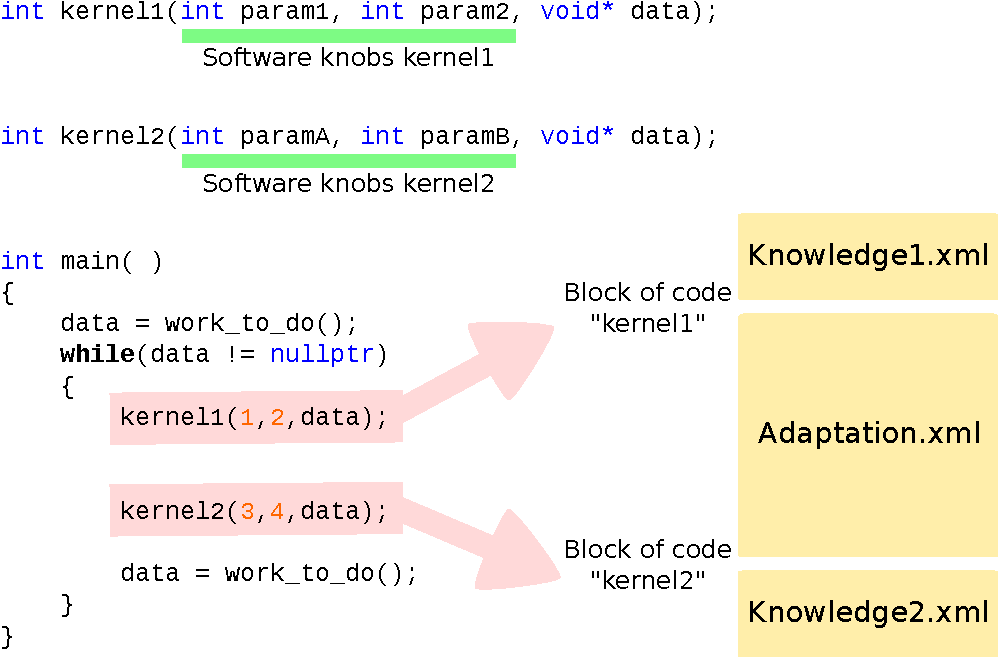
\includegraphics[scale=0.5]{code_example1}
\caption{Pseudo-code of an application with two block of code to be tuned.}
\label{fig:code_example1}
\end{figure}


To clarify the concept, \prettyref{fig:code_example1} shows a pseudo-code of a very simple application.
The whole computation is a loop that executes two different kernels on the same data.
In this example we suppose that the developer is interested on managing two different blocks of the application (highlighted in red).
The first block is named ``kernel1'', while the second block is named ''kernel2''.
We would like to stress the fact that a block of code might involve several lines of code, not just a function call.
In this case we have a single configuration file for the Monitor and Plan elements (\textit{Adaptation.xml}) of both the blocks of code; while we have two different files for the application Knowledge (\textit{Knowledge1.xml} and \textit{Knowledge2.xml}).

\section{Knowledge configuration file}
\label{sec:knowledge}


The configuration file that describes the application knowledge must be a different file with respect to the one that describes extra-functional concerns, to ensure separation of concerns.
The structure of the configuration file matches the application knowledge representation of mARGOt.
In particular, it is a list of Operating Points (OPs), where each OP has up to three fields:
\begin{enumerate}
	\item The feature section (if any)
	\item The software-knobs section
	\item The metric section
\end{enumerate}
The feature section states the value for each input feature field.
Since mARGOt use input features as indipedent cluster of Operating Point, a best practice would be to ensure that all the input feature clusters contain OPs with the same configurations of software-knobs.

Each section of the OP is basically a key-value pair, where the key is the name of field and the value is a number, which represents its average value.
In the software-knob section, the field can be a string.
In the metric section, we can use two values to define the mean and standard deviation of the related distribution.
These two exceptions are enabled by the the extra-functional concerns stated in the mARGOt configuration file, explained in details in \prettyref{sec:adaptation}.

\begin{figure}
\lstset{language=json}
\begin{lstlisting}
{
	"foo":
	[
		{
			"features": { "resolution": 34 },
			"knobs": { "threads": 3, "algorithm": "one" },
			"metrics": { "throughput": [23.0, 2.0], "quality": 32 }
		},
		{
			"features": { "resolution": 34 },
			"knobs": { "threads": 4, "algorithm": "two" },
			"metrics": { "throughput": [2.0, 0.5], "quality": 100 }
		}
	]
}
\end{lstlisting}
\caption{Example of a knowledge configuration file for a block named ``foo''.}
\label{code:knowledge_file}
\end{figure}


\prettyref{code:knowledge_file} shows an example of the syntax of the knowledge file, that defines an Operating Point list for a block named ``foo'', by defining a root element with the same name that will contain the OP list.
A configuration file that represents the application knowledge may contain more than one OP list, if the application is composed of more than one block of code.
However, this behaviour is not recommended to ensure separation of concerns.
The application knowledge of a block of code can be splitted in more than file, to limit its size.
In this example, we have just a single input feature named ``resolution'', defined in the element with tag \textbf{features}.
If we don't have any input feature, the \textbf{features} element can be omitted.
We have two software-knobs, named ``threads'' and ``algorithm'', defined in the element with tag \textbf{knobs}.
The values of the second knob are strings.
Finally, we have two metrics, named ``throughput'' and ``quality'', defined in the element with tag \textbf{metrics}.
For the metric ``quality'', the average value is enough to describe the reached performance.
It may happen when the metric is determistic.
Instead, the metric ``throughput'' is a distribution defined by an average value and the standard deviation.
While the OPs that belong to the same block managed by mARGOt have the same structure, the actual values changes to define the application knowledge.



\section{Adaptation file overview}

\begin{figure}
\lstset{language=XML}
\begin{lstlisting}
<margot>

	<block name="kernel1">
		<!-- The configuration of block kernel1: -->
		<!--    - Description of the Monitor element -->
		<!--    - Description of the Plan element -->
	</block>
	
	<block name="kernel2">
		<!-- The configuration of block kernel2: -->
		<!--    - Description of the Monitor element -->
		<!--    - Description of the Plan element -->
	</block>

</margot>
\end{lstlisting}
\caption{Minimal adaptation configuration file.}
\label{code:min_adaptation}
\end{figure}

This section describes the adaptation XML file, which define the Monitor and Plan elements for every block of code that will be tuned by mARGOt.
The root element of the XML configuration file is the \textit{margot} tag, which holds the definition of all the block of code of the application.
The configuration of each block of code is inserted in the \textit{block} tag, which has also the attribute \textit{name} which holds the name of the block of code.
The name of the block must be a valid C++ namespace identifier.
\prettyref{code:min_adaptation} shows a simple example on how it is possible to generate an empty configuration for the blocks depicted in \prettyref{fig:code_example1}.

Since each block of code is independent from each other, in the remainder of the documentation we focus only in a single block of code, without losing in generality.


\subsection{Describing the monitor element}
\label{ssec:monitor_element}

The description of the Monitor elements consists in the list of Monitors that observe a metric of interest for the developer.
The mARGOt framework ships with a suite of monitors for the most common metrics.
However, the configuration file is able to handle custom monitors as well.


\begin{figure}
\lstset{language=XML}
\begin{lstlisting}
<monitor name="my_custom_monitor" type="custom">

	<spec>
		<header reference="my_monitor.hpp" />
		<class name="MyCustomMonitor" />
		<type name="double" />
		<stop_method name="my_stop" />
		<start_method name="my_start" />
	</spec>
	
	<creation>
		<param name="window_size">
			<fixed value="1" />
		</param>
	</creation>
	
	<start>
		<param>
			<local_var name="start_param" type="int" />
		</param>
	</start>

	<stop>
		<param name="error">
			<local_var name="error" type="double" />
		</param>
	</stop>

	<expose var_name="avg_quality" what="average" />

</monitor>
\end{lstlisting}
\caption{Example of the definition of a monitor element.}
\label{code:monitor_xml}
\end{figure}


In particular, \prettyref{code:monitor_xml} shows an example of the full declaration of a monitor that observe a metric of interest.
Each tag \textit{monitor} states the characteristic of the monitor of interested and it must specify the identifier of the monitor (with the attribute \textit{name}) and its type (with the attribute \textit{type}).
The identifier of the monitor must be a valid C++ identifier.
The type of the monitor is an enumeration of all the available monitor in mARGOt, plus the \textit{custom} enumerator which represents a user-defined monitor.


In current implementation, the available monitor in mARGOt are:
\begin{enumerate}
	\item[Frequency] For the frequency monitor
	\item[Memory] For the memory monitor
	\item[PAPI] For the PAPI monitor
	\item[CPUPROCESS] For the process CPU usage monitor
	\item[CPUSYSTEM] For the system-wide CPU usage monitor
	\item[Temperature] For the temperature monitor
	\item[Throughput] For the throughput monitor
	\item[Time] For the time monitor
	\item[Collector] For the ETHz monitoring framework
	\item[ENERGY] For the energy monitor, using RAPL
	\item[ODROID\_POWER] For the power monitor on Odroid
	\item[ODROID\_ENERGY] For the energy monitor on Odroid
\end{enumerate}


The type of the monitor is not case sensitive.
If the type of the monitor is \textit{custom}, it means that the developer is planning to use a monitor which is not shipped with the framework.
For this reason it should specify also the monitor specification from a C++ point of view.
The latter is defined within the XML tag \textit{spec}.
In particular, the developer should specify:
\begin{enumerate}
	\item The header of the C++ which define the monitor object, using the \textit{reference} attribute of the XML tag \textit{header}
	\item The name of the C++ class, using the \textit{name} attribute of the XML element \textit{class}
	\item The type of the observed values stored in the monitor, using the \textit{name} attribute of the XML tag \textit{type}
	\item If any, the name of the method that starts a measure, using the attribute \textit{name} of the XML tag \textit{start\_method}
	\item If any, the name of the method that stops a measure, using the attribute \textit{name} of the XML tag \textit{stop\_method}
\end{enumerate}

The remainder of the specification for the monitor have two purposes: defining the \textbf{input} and \textbf{output} variables for the monitor.
In particular, the XML tag \textit{creation} states all the parameters of the C++ constructor of the monitor.
The XML tag \textit{start} states all the parameters of the C++ method that starts a measure.
Finally, the XML tag \textit{stop} states all the parameters of the C++ method that stops a measure.

Syntactically, all the parameters are specified by the XML tag \textit{param}, however its actual content depends on the nature of the parameter.
In particular, if the parameter is an immediate value, then it is represented by the attribute \textit{value} of the XML tag \textit{fixed}.
If the parameter must be an l-value or it is not known at compile time, it is possible to forward its value to the developer, relying on function parameters exposed to the developer.
In this case the developer must specify the XML tag \textit{local\_var}, which is defined by the C++ type of the parameter (using the attribute \textit{type}) and the name of the parameter (using the attribute \textit{name}).
Semantically, the parameters depends on the monitor, see \prettyref{appendix:monitor_implementation} for a complete list of parameter for each monitor shipped with mARGOt.

Since each monitor collects the observations in a circular buffer, the output variables for the monitor are the statistical properties of interest for the developer (i.e. the average).
The XML tag \textit{expose} identifies such property.
In particular the attribute \textit{name} states the name of the variable that holds such value (therefore it must be a valid C++ identifier), while the attribute \textit{what} identify the target statistical property.
The following is the list of the available statistical properties:
\begin{enumerate}
	\item[AVERAGE] To retrieve the mean value of the observations.
	\item[STDDEV] To retrieve the standard deviation of the observations.
	\item[MAX] To retrieve the maximum value of the observations.
	\item[MIN] To retrieve the minimum value of the observations.
\end{enumerate}


\subsection{Describing the geometry of the application knowledge}


\begin{figure}
	\lstset{language=XML}
	\begin{lstlisting}
	<!-- SW-KNOB SECTION -->
	<knob name="num_threads" var_name="threads" var_type="int"/>
	<knob name="num_trials" var_name="trials" var_type="int"/>
	
	<!-- METRIC SECTION -->
	<metric name="throughput" type="float" distribution="yes"/>
	<metric name="quality" type="float" distribution="no"/>
	
	<!-- FEATURE SECTION -->
	<features distance="euclidean">
		<feature name="size_x" type="int" comparison="LE"/>
		<feature name="size_y" type="int" comparison="-"/>
	</features>
	
	\end{lstlisting}
	\caption{Example of definition for the geometry of the application knowledge.}
	\label{code:geometry_xml}
\end{figure}

The autotuning framework leverage as much as possible, compile-time information to specialize the definition of the manger.
In particular, it requires to know the geometry of the application knowledge, i.e. the software knobs, the metrics of interest and the data features (if any).
Without those information, it is possible to use the high-level interface for profiling purpose, but no manager will be instantiated.


\subsubsection*{Software-knob section}

This section relates the software-knob states in the application knowledge, with C++ variables that must be exported to the application in the update function.
In particular, each software knob is represented by the XML tag \textit{knob} and must define:
\begin{itemize}
	\item the attribute \textit{name}, which relates to the name of a software knob in the application knowledge
	\item the attribute \textit{var\_name}, which is the name of the exported variable, therefore it must be a valid C++ identifier.
	\item the attribute \textit{var\_type}, states the C++ type of the exported variable.
\end{itemize}

These information -- together with the the data features (if any) --  are used to compose the signature of the update function, exposed to the user.

\subsubsection*{Metric section}

This section define the metrics of interest.
In particular, each metric is represented by the XML tag \textit{metric} and must define:
\begin{itemize}
	\item the attribute \textit{name}, which attach a label to the metric index
	\item the attribute \textit{type}, shall define the minimum C-type required to express the metric in the application knowledge.
	\item the attribute \textit{distribution}, which states whether the metric is a distribution or not. If a metric is declared as distribution, the application knowledge shall define also the standard deviation of the metric. If a metric is not declared as distribution, any information about its standard deviation in the application knowledge is discarded.
\end{itemize}

Heterogeneous metrics will be automatically handled when the high-level library is generated. 



\subsubsection*{Feature section}

This section is optional and defines the input features of the block of code and how to handle them.
In particular, all the features are represented by the XML tag \textit{features}.
The latter shall define the attribute \textit{distance}, which states how the framework should compute the distance between data features.
In the current version, the available values are:
\begin{itemize}
	\item[NORMALIZED] For computing a normalized distance between data feature, useful if the data features have values which differs by orders of magnitudes
	\item[EUCLIDEAN] For computing a classic euclidean distance. 
\end{itemize}

As child of the \textit{features} element, each XML tag \textit{feature} represents a data feature.
The latter element shall define:
\begin{itemize}
	\item the attribute \textit{name}, which relates to the name of a software knob in the application knowledge and the name of the variable exposed to the update function. Therefore should be a valid C identifier.
	\item the attribute \textit{type}, shall define the minimum C-type required to express the metric in the application knowledge. This will be also the type of the variable exposed to the update function.
	\item the attribute \textit{comparison}, which states the validity comparison for the defining data feature. It might assume the following values:
	\begin{itemize}
		\item[GE] To express the fact that the defining data feature of the selected feature cluster must be greater or equals to the value of the current input.
		\item[LE] To express the fact that the defining data feature of the selected feature cluster must be less or equals to the value of the current input.
		\item[-] To express the fact that there is no validity requirement for the defining data feature.
	\end{itemize}
\end{itemize}


These information -- together with the software knobs --  are used to compose the signature of the update function, exposed to the user.


\subsection{Describing the plan element}

The main goal of the plan element to state the concept of ``best'' for the application developer.
Internally, mARGOt represent such definition as a constrained multi-objective optimization problem.
Since the application might have different definitions of ``best'', according to its evolution or external events, it is possible to state more than one optimization problem (or states in mARGOt context). 



\begin{figure}
\lstset{language=XML}
\begin{lstlisting}
<!-- GOAL SECTION -->
<goal name="threads_g" knob_name="num_threads" cFun="LT" value="2" />
<goal name="quality_g" metric_name="quality" cFun="LT" value="80" />

<!-- RUNTIME INFORMATION PROVIDER -->
<adapt metric_name="exectime" using="my_time_monitor" inertia="1" />

<!-- OPTIMIZATION SECTION -->
<state name="my_optimization_1" starting="yes" >
	<minimize combination="linear">
		<knob name="num_threads" coef="1.0"/>
		<metric name="exectime" coef="2.0"/>
	</minimize>
	<subject to="quality_g" priority="30" />
</state>

<state name="my_optimization_2" >
	<maximize combination="geometric">
		<metric name="quality" coef="1.0"/>
	</maximize>
	<subject to="threads_g" priority="10" />
	<subject to="exectime_g" priority="20" confidence="3" />
</state>

\end{lstlisting}
\caption{Example of the definition of the plan element.}
\label{code:plan_xml}
\end{figure}

\prettyref{code:plan_xml} shows an example of a definition of a plan element.
In particular, it includes the definition of two sections: the goal section and the optimization section.
These two sections are related with each other, with the geometry of the application knowledge, the monitors stated in the definition of the monitor element and the application knowledge.
The remainder of this section explains in details such relations.

\subsubsection*{Goal section}
\label{ssec:goal}

This section states all the goals that the developer would like to express.
Each goal represents a target that must be reached (i.e. \textit{$<subject>$} must be \textit{$<comparison_function>$} than \textit{$<value>$})
The mere definition of a goal does not influence the selection of the configuration.

A goal is represented by the XML tag \textit{goal}.
The attribute \textit{name} identify the goal and it has to be a valid C++ identifier.
The attribute \textit{value} states the actual numeric value of the goal.
The attribute \textit{cFun} states the comparison function of the goal.
The available comparison functions are:
\begin{enumerate}
	\item[GT] For the ``greater than'' comparison function.
	\item[GE] For the ``greater or equal than'' comparison function.
	\item[LT] For the ``less than'' comparison function.
	\item[LE] For the ``less or equal than'' comparison function. 
\end{enumerate}

For the generation of the high-level interface, the goal subject is a field (either a metric or a software-knob) of the application knowledge.
In particular, if the goal targets a metric, it must define the attribute \textit{metric\_name}, which holds the name of a metric in the related Operating Point (see \prettyref{sec:knowledge}).
If the goal targets a software-knob, it must define the attribute \textit{knob\_name}, which holds the name of a software-knob in the related Operating Point.


\subsubsection*{Runtime adaptation section}

This section states all the feedback loops required by the application developer.
In particular, mARGOt might use runtime information from the monitors to adapt the application knowledge.
Therefore, it is possible to state that a given metric is observed by the related monitor by using the XML tag \textit{adapt}.
The latter XML element shall define the following attributes:
\begin{itemize}
	\item \textit{metric\_name} to identify the target metric in the application knowledge geometry. In particular, its value shall be the name of a metric stated in the metrics section.
	\item \textit{using} to identify the target monitor. In particular, its value shall be the name of the monitor stated in the monitors section.
	\item \textit{inertia} to define the inertia of the adaptation. This field shall be a positive integer number.
\end{itemize} 




\subsubsection*{Optimization section}

This section states the list of states, which is the list of constrained multi-objective optimization problems.
In particular, each state is represented by the XML tag \textit{state}, using the attribute \textit{name} to identify it.
If the developer specify more than one state, he also have to specify which is the starting state, using the attribute \textit{starting} and setting its value to ``yes''.


Each state is composed by an objective function that must be maximized or minimized and the list of constraints.
The objective function is represented by either the XML tag \textit{maximize} or \textit{minimize}, according to the requirements of the application.
Since the objective function is a composition of fields (thus metrics and/or knobs), the attribute \textit{combination} specify the composition formula.
In the current implementation are available two kind of compositions:
\begin{enumerate}
	\item a geometrical combination, represented by the value ``geometric''
	\item a linear combination, represented by the value ``linear''
	\item a simple combination, i.e. it targets only a single field, represented by the value ``simple''
\end{enumerate}
As child  of the objective function tag, there is the list of fields that compose the objective function.
In particular, the XML tag \textit{metric} represents a metric of the application knowledge, specified by the attribute \textit{name}; while the XML tag \textit{knob} represents a software-knob of the application knowledge, specified by the attribute \textit{name}.
Both cases require to define the attribute \textit{coefficient}, which states the numeric value of the coefficient of each term in the combination.
This hold true also in case of a ``simple'' combination.


The list of constraints is represented by the list of XML tags \textit{subject}, using the attribute \textit{to} to specify the related goal name (see \prettyref{ssec:goal}), the attribute \textit{priority} to specify the priority of constraint and (optionally) the attribute \textit{confidence} to specify the confidence level of the constraint.
The priority is a number used to order by importance the constraints, therefore it is required that each constraint of a state must have a different priority.
If the constraints relates to a goal whose subject is a monitored value, it is required to specify the name of the related metric in the application knowledge, using the attribute \textit{metric\_name}.
The confidence is the number of times to take into account the standard deviation in the Operating Point evaluation, therefore it must be an integer number.






















\section{mARGOt command line interface}

The mARGOt command line interface (margot\_cli) is a python script to provide to the end-user utility functions to manage the mARGOt heel configuration files.
The usage of the script is explained in the its help command.
The most important command is \textit{generate} which automatically generates the source code of the high level interface, from the XML configurations files.
This is the command  leveraged by margot\_if to generate the high-level interface library.
Beside this command, margot\_cli expose the following operations to manage the application knowledge:
\begin{itemize}
	\item[plotOPs] It takes in input the XML configuration file of the application knowledge and it prints on the standard output a gnuplot script that display the application knowledge, according to the fields specified at command line.
	\item[pareto] It takes in input the XML configuration file of the application knowledge and it prints on the standard output the XML configuration file of application knowledge with only the Operating Points which belong to the Pareto set, according to the criteria specified at command line.
	\item[csv2xml] It takes in input the CSV configuration file of the application knowledge and it prints on the standard output the XML configuration file of application knowledge.
	\item[xml2csv] It takes in input the XML configuration file of the application knowledge and it prints on the standard output the CSV configuration file of application knowledge
\end{itemize}

The CSV format of the application knowledge shall represents the Operating Point list using the following conventions.
Each row is considered a different Operating Point.
Each column is considered a field of the Operating Point.
All the column of the file shall have an header to identify the field:
\begin{itemize}
	\item Each software knob shall have the prefix ``\#''. For example, to represent the knob ``compiler\_flag'', the header name should be ``\#compiler\_flag''.
	\item The metric mean value and standard deviation must be in two separated columns. In particular, the column with the mean value of the metric is written in plain, while its standard deviation shall have the ``\_standard\_dev'' suffix. For example to represent the mean value and the standard deviation of the metric execution time, the header of the column that represents the mean value is ``exec\_time'', while the header of the column that represents its standard deviation is ``exec\_time\_standard\_dev``.
	\item Each data feature shall have the prefix ``$@$''. For example, to represent the data feature ``size'', the header name should be ``$@$size''.
\end{itemize}

All the required suffixes and prefixes will be stripped from the actual name of the field.


% Set the appendix
\clearpage
\pagenumbering{roman}
\setcounter{page}{1}
\appendix
\section{Monitor implementation details}
\label{appendix:monitor_implementation}

This appendix lists, for each monitor, all the parameters of its constructor, start measure method and stop measure method.
These information might be used when a monitor is declared in the XML configuration file.



\subsection{Collector Monitor}

\subsubsection*{Constructor parameters}
\begin{enumerate}
	\item Default constructor
		\begin{itemize}
			\item Size of the observation window (default = 1)
			\item Minimum number of observations (default = 1)
		\end{itemize}
	\item Custom connection constructor
		\begin{itemize}
			\item Name of the topic of interest (string)
			\item Address of the MQTT broker (string)
			\item Size of the observation window (default = 1)
			\item Minimum number of observations (default = 1)
		\end{itemize}
\end{enumerate}

\subsubsection*{Start method parameters}
\begin{enumerate}
	\item[] N/A
\end{enumerate}


\subsubsection*{Stop method parameters}
\begin{enumerate}
	\item[] N/A
\end{enumerate}






\subsection{Energy Monitor}

\subsubsection*{Constructor parameters}
\begin{enumerate}
	\item Default constructor
		\begin{itemize}
			\item Size of the observation window (default = 1)
			\item Minimum number of observations (default = 1)
		\end{itemize}
	\item Custom domain constructor
		\begin{itemize}
			\item Domain of interest
				\begin{enumerate}
					\item margot::EnergyMonitor::Domain::Cores
					\item margot::EnergyMonitor::Domain::Uncores
					\item margot::EnergyMonitor::Domain::Ram
					\item margot::EnergyMonitor::Domain::Package
				\end{enumerate}
			\item Size of the observation window (default = 1)
			\item Minimum number of observations (default = 1)
		\end{itemize}
\end{enumerate}

\subsubsection*{Start method parameters}
\begin{enumerate}
	\item[] N/A
\end{enumerate}


\subsubsection*{Stop method parameters}
\begin{enumerate}
	\item[] N/A
\end{enumerate}





\subsection{Frequency Monitor}

\subsubsection*{Constructor parameters}
\begin{enumerate}
	\item Default constructor
		\begin{itemize}
			\item Size of the observation window (default = 1)
			\item Minimum number of observations (default = 1)
		\end{itemize}
\end{enumerate}

\subsubsection*{Start method parameters}
\begin{enumerate}
	\item[] N/A
\end{enumerate}


\subsubsection*{Stop method parameters}
\begin{enumerate}
	\item[] N/A
\end{enumerate}




\subsection{Odroid Energy Monitor}

\subsubsection*{Constructor parameters}
\begin{enumerate}
	\item Default constructor
		\begin{itemize}
			\item Size of the observation window (default = 1)
			\item Minimum number of observations (default = 1)
		\end{itemize}
	\item Custom period time
		\begin{itemize}
			\item Period of polling (unsigned integer)
			\item Size of the observation window (default = 1)
			\item Minimum number of observations (default = 1)
		\end{itemize}
\end{enumerate}

\subsubsection*{Start method parameters}
\begin{enumerate}
	\item[] N/A
\end{enumerate}


\subsubsection*{Stop method parameters}
\begin{enumerate}
	\item[] N/A
\end{enumerate}




\subsection{Odroid Power Monitor}

\subsubsection*{Constructor parameters}
\begin{enumerate}
	\item Default constructor
		\begin{itemize}
			\item Size of the observation window (default = 1)
			\item Minimum number of observations (default = 1)
		\end{itemize}
\end{enumerate}

\subsubsection*{Start method parameters}
\begin{enumerate}
	\item[] N/A
\end{enumerate}


\subsubsection*{Stop method parameters}
\begin{enumerate}
	\item[] N/A
\end{enumerate}






\subsection{Papi Monitor}

\subsubsection*{Constructor parameters}
\begin{enumerate}
	\item Trivial Default constructor
		\begin{itemize}
			\item[] N/A
		\end{itemize}
	\item Custom event constructor
		\begin{itemize}
			\item PAPI event of interest
				\begin{enumerate}
					\item margot::PapiEvent::L1\_MISS
					\item margot::PapiEvent::L2\_MISS
					\item margot::PapiEvent::L3\_MISS
					\item margot::PapiEvent::INS\_COMPLETED
					\item margot::PapiEvent::NUM\_BRANCH
					\item margot::PapiEvent::NUM\_LOAD
					\item margot::PapiEvent::NUM\_STORE
					\item margot::PapiEvent::CYC\_NO\_ISSUE
					\item margot::PapiEvent::CYC\_TOT
				\end{enumerate}
			\item Size of the observation window (default = 1)
			\item Minimum number of observations (default = 1)
		\end{itemize}
\end{enumerate}

\subsubsection*{Start method parameters}
\begin{enumerate}
	\item[] N/A
\end{enumerate}


\subsubsection*{Stop method parameters}
\begin{enumerate}
	\item[] N/A
\end{enumerate}








\subsection{Process CPU Usage Monitor}

\subsubsection*{Constructor parameters}
\begin{enumerate}
	\item Default constructor
		\begin{itemize}
			\item Size of the observation window (default = 1)
			\item Minimum number of observations (default = 1)
		\end{itemize}
	\item Custom CPU time counter constructor
		\begin{itemize}
			\item CPU time counter
				\begin{enumerate}
					\item margot::CounterType::SoftwareCounter
					\item margot::CounterType::HardwareCounter
				\end{enumerate}
			\item Size of the observation window (default = 1)
			\item Minimum number of observations (default = 1)
		\end{itemize}
\end{enumerate}

\subsubsection*{Start method parameters}
\begin{enumerate}
	\item[] N/A
\end{enumerate}


\subsubsection*{Stop method parameters}
\begin{enumerate}
	\item[] N/A
\end{enumerate}




\subsection{System CPU Usage Monitor}

\subsubsection*{Constructor parameters}
\begin{enumerate}
	\item Default constructor
		\begin{itemize}
			\item Size of the observation window (default = 1)
			\item Minimum number of observations (default = 1)
		\end{itemize}
\end{enumerate}

\subsubsection*{Start method parameters}
\begin{enumerate}
	\item[] N/A
\end{enumerate}


\subsubsection*{Stop method parameters}
\begin{enumerate}
	\item[] N/A
\end{enumerate}



\subsection{Temperature Monitor}

\subsubsection*{Constructor parameters}
\begin{enumerate}
	\item Default constructor
		\begin{itemize}
			\item Size of the observation window (default = 1)
			\item Minimum number of observations (default = 1)
		\end{itemize}
\end{enumerate}

\subsubsection*{Start method parameters}
\begin{enumerate}
	\item[] N/A
\end{enumerate}


\subsubsection*{Stop method parameters}
\begin{enumerate}
	\item[] N/A
\end{enumerate}




\subsection{Throughput Monitor}

\subsubsection*{Constructor parameters}
\begin{enumerate}
	\item Default constructor
		\begin{itemize}
			\item Size of the observation window (default = 1)
			\item Minimum number of observations (default = 1)
		\end{itemize}
\end{enumerate}

\subsubsection*{Start method parameters}
\begin{enumerate}
	\item[] N/A
\end{enumerate}


\subsubsection*{Stop method parameters}
\begin{enumerate}
	\item Amount of data processed (float)
\end{enumerate}





\subsection{Time Monitor}

\subsubsection*{Constructor parameters}
\begin{enumerate}
	\item Default constructor
		\begin{itemize}
			\item Size of the observation window (default = 1)
			\item Minimum number of observations (default = 1)
		\end{itemize}
	\item Custom time unit constructor
		\begin{itemize}
			\item Time resolution
				\begin{enumerate}
					\item margot::TimeUnit::NANOSECONDS
					\item margot::TimeUnit::MICROSECONDS
					\item margot::TimeUnit::MILLISECONDS
					\item margot::TimeUnit::SECONDS
				\end{enumerate}
			\item Size of the observation window (default = 1)
			\item Minimum number of observations (default = 1)
		\end{itemize}
\end{enumerate}

\subsubsection*{Start method parameters}
\begin{enumerate}
	\item[] N/A
\end{enumerate}


\subsubsection*{Stop method parameters}
\begin{enumerate}
	\item[] N/A
\end{enumerate}



\end{document}
